\documentclass[12pt,twoside]{article}			
\usepackage[utf8]{inputenc}	% az alábbi 3 sor az ékezetes betűkhöz
\usepackage[T1]{fontenc}
\usepackage{lmodern}
\usepackage{pifont}
\usepackage{fancyhdr} % header és footer kezeléshez
\usepackage[hungarian]{babel} % magyar szótagoláshoz
\usepackage{graphicx} % képek
\usepackage[dvipsnames]{xcolor}
\usepackage{pdfpages}
\usepackage{cite}
\usepackage{enumerate} %listázáshoz
\usepackage{amsmath}
\usepackage{eqnarray}
\usepackage{gensymb} %\degree
\usepackage{float} %[H]
\usepackage{mathtools}
\usepackage{hyperref}
\hypersetup{colorlinks=false,pdfborder={0 0 0},}
\usepackage[a4paper, top=1in, bottom=1in, left=1in, right=1in]{geometry} %margókhoz
\usepackage[bold]{hhtensor} % matrix, vector
\usepackage{tabularx}%fancy táblázatokhoz
\usepackage{comment}

\newcommand{\pd}[2]{\frac{\partial #1}{\partial #2}}


\pagestyle{fancy}
\fancyhf{}
\fancyhead[LE,RO]{Váncza Tihamér}
\fancyfoot[LE,RO]{\thepage}
\setlength\parindent{0pt}




\begin{document}


Munka dokumentáció 

 \section{Kisebb rendszerek modellezése }
 
\subsection{1DoF, csillapítatlan, nem követő erő} %1.1__________________________________
\begin{figure}[H]
\center
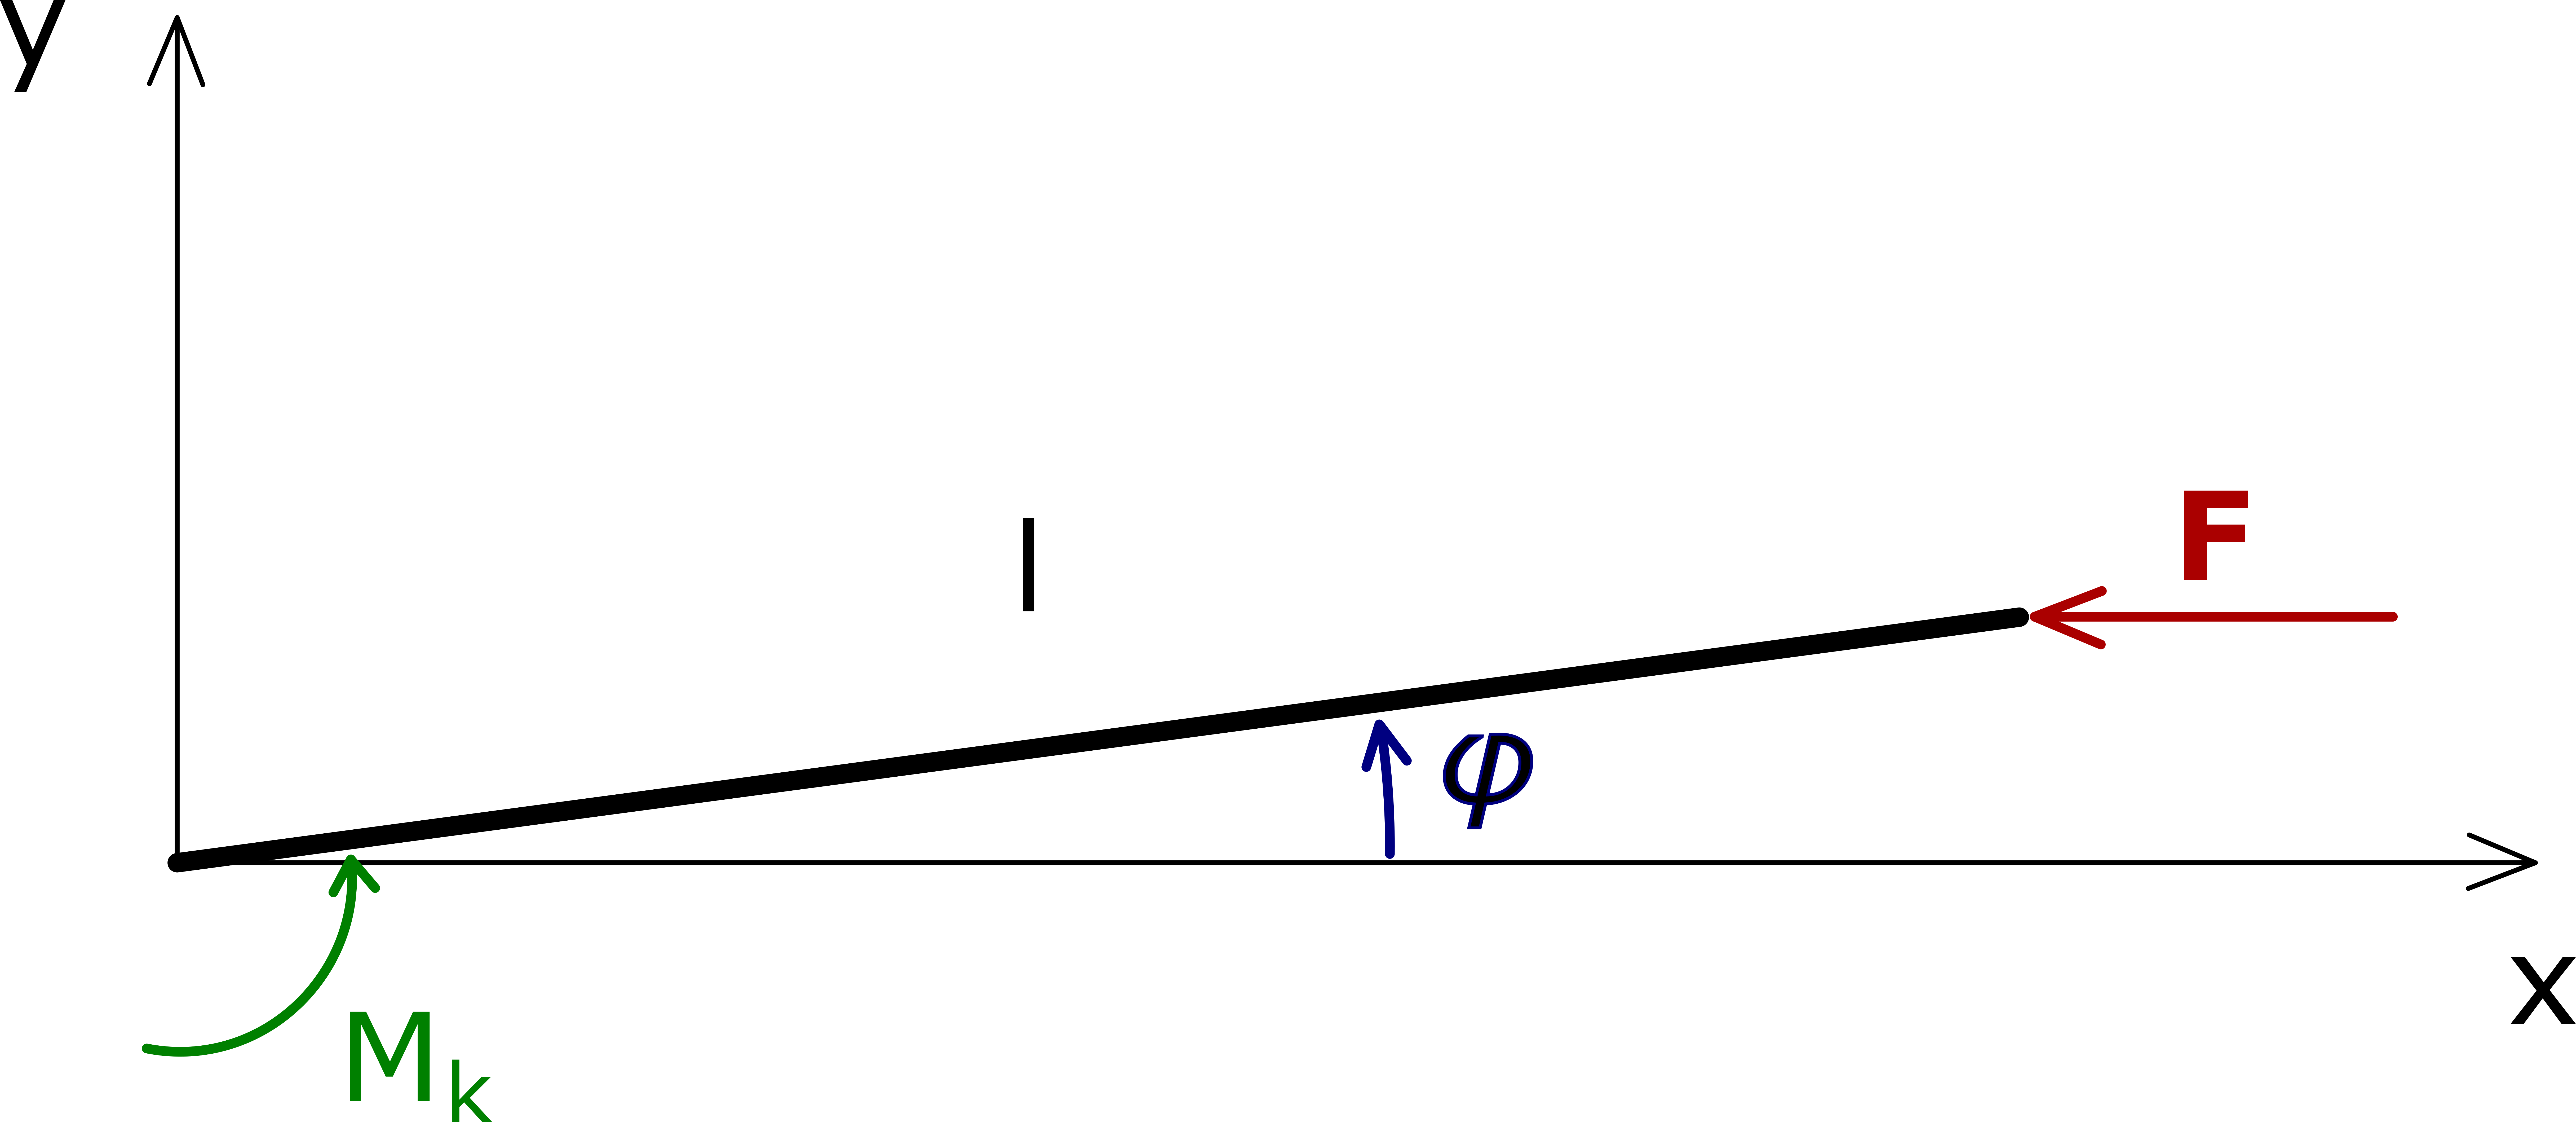
\includegraphics[scale=1]{1szab_nem_koveto}
\end{figure}
 Jelölje a rugó merevségét \emph{k}, a rúd hosszát \emph{l}, az erő nagyságát \emph{F}. Legyen $  k>0, l>0, F>0 $  \newline
 A rendszer konzervatív, és csillapítatlan, gerjesztetlen, ezért ha a potenciálfüggvénynek a $  \varphi =0 $ pontban lokális minimuma van, akkor a $  \varphi \rightarrow 0,  \dot \varphi \rightarrow 0, $ kezdeti állapotból induló rendszerek stabilak lesznek. A rúd tömege - tehetetlenségi nyomatéka a stabilitásra nincs, csak a rezgés frekvenciájára van hatással, ezért ezzel most nem foglalkozom. \newline
A potenciálfüggvény az alábbi alakban írható fel felírható:
\begin{equation} \label{eq:Newton}
U(\varphi)=k/2 \cdot \varphi ^2 + F l \cdot ( cos\varphi-1)
\end{equation}
 \begin{equation} \label{eq:Newton}
U'(0)=k \cdot 0 - F l \sin0=0 ; \;
U''(0)=k  - F l \cos0=k-Fl ; \;
\end{equation}
\begin{equation} \label{eq:Newton}
U'''(0)=\sin0=0;\;
U''''(0)=Fl\cos0=Fl
\end{equation}
$  k>0, l>0, F>0 $ Ezért $  k [Nm/rad]\geq F[N] \cdot l [m] $ esetén a rendszer stabil $  \varphi =0 $ körül, egyébb esetben instabil.

\subsection{2DoF, csillapítatlan, nem követő erő} %1.2____________________________________
\begin{figure}[H]
\center
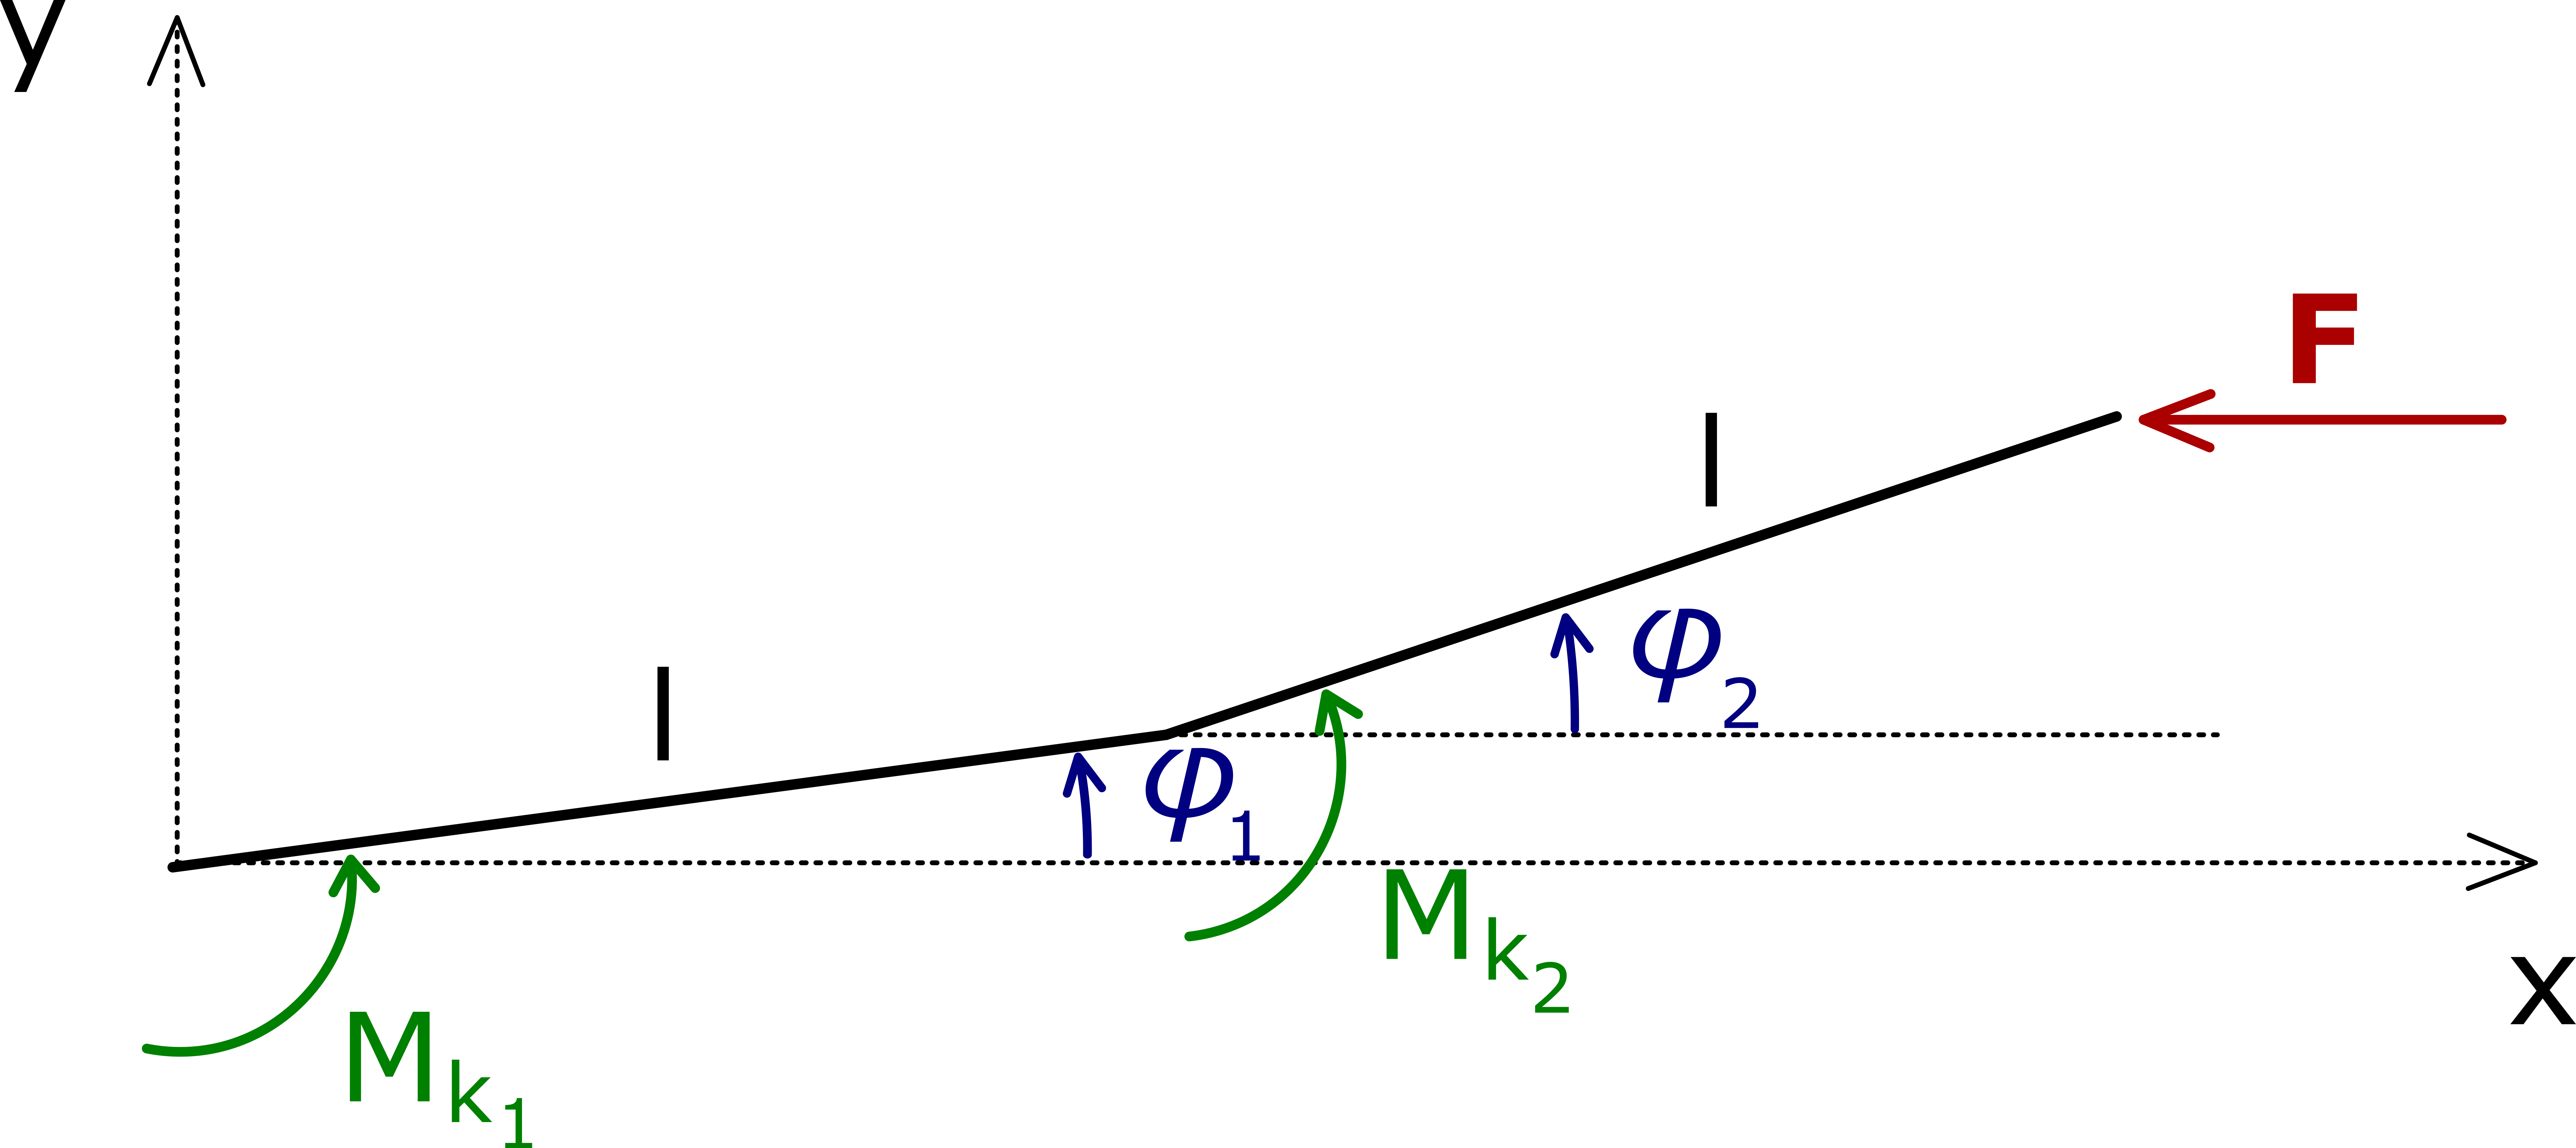
\includegraphics[scale=1]{2szab_nem_koveto}
\end{figure}
Jelölje a rugók merevségét $  k_1=k_2=k>0 $, a rúdak hosszát $  l_1=l_2=l>0 $, az erő nagyságát \emph{F}. Legyen $ k>0, l>0, F>0 $  \newline
A rendszer konzervatív, és csillapítatlan, gerjesztetlen, így az előző gondolatmenet alapján elég a potenciálfüggvényt vizsgálni. \newline
A potenciálfüggvény az alábbi alakban írható fel felírható:
\begin{equation} \label{eq:Newton}
U(\vec\varphi)=k/2 \cdot \varphi_1 ^2 + k/2 \cdot (\varphi_2- \varphi_1) ^2 +F l \cdot ( \cos\varphi_1+ \cos\varphi_2 -2)
\end{equation}
A potenciál függvény első, és második deriváltjai:
\begin{equation} \label{eq:Newton}
\vec Q(\vec\varphi) =[k_{i}]=\left[ \frac{\partial U}{\partial \varphi_i }\right]=
\begin{bmatrix}
2k \varphi_1 - k \varphi_2-Fl\sin\varphi_1\\
k \varphi_2 - k \varphi_1-Fl\sin\varphi_2
\end{bmatrix}
\end{equation}
\begin{equation} \label{eq:Newton}
\matr K(\vec\varphi) =[k_{ij}]=\left[ \frac{\partial^2 U}{\partial \varphi_i \partial \varphi_j}\right]=
\begin{bmatrix}
2k-Fl \cos\varphi_1 & -k \\
-k & k-Fl \cos\varphi_2 
\end{bmatrix}
\end{equation}
$\vec{Q}(\vec0)=\vec0$, tehát $\vec\varphi = \vec0$ a rendszernek egyensúlyi helyzete, $\vec K(\vec0)$ előjeles aldeterminánsainak előjelén múlik, hogy ez az egyensúlyi helyzet stabil-e.\newline
$\vec K(\vec0)$ előjeles aldeterminánsai:
\begin{equation} \label{eq:Newton}
K_{aldet 1}=2k-Fl
\end{equation}
\begin{equation} \label{eq:Newton}
K_{aldet 2}=(2k-Fl)(k-Fl)-k^2=k^2-3kFl+F^2l^2
\end{equation}
$  \vec\varphi=\vec0  $ stabil pont ha:
\begin{equation} \label{eq:Newton}
2k>Fl; \; k^2-3kFl+F^2l^2>0  \Leftrightarrow \left(\frac{3k+\sqrt{5}k}{2}-Fl\right)\left(\frac{3k-\sqrt{5}k}{2}-Fl\right)>0
\end{equation}
  $ k>0 , Fl>0$ felhasználásával, és mivel $3+\sqrt5>4$
\begin{equation} \label{eq:Newton}
\frac{3-\sqrt{5}}{2}k>Fl \Leftrightarrow 0,382k>Fl
\end{equation}

0,382k>Fl esetén a rendszernek $\vec\varphi = \vec 0$ stabil pontja.


\section{2DoF, csillapítatlan, követő erő}%2______________________________________________
\begin{figure}[H]
\center
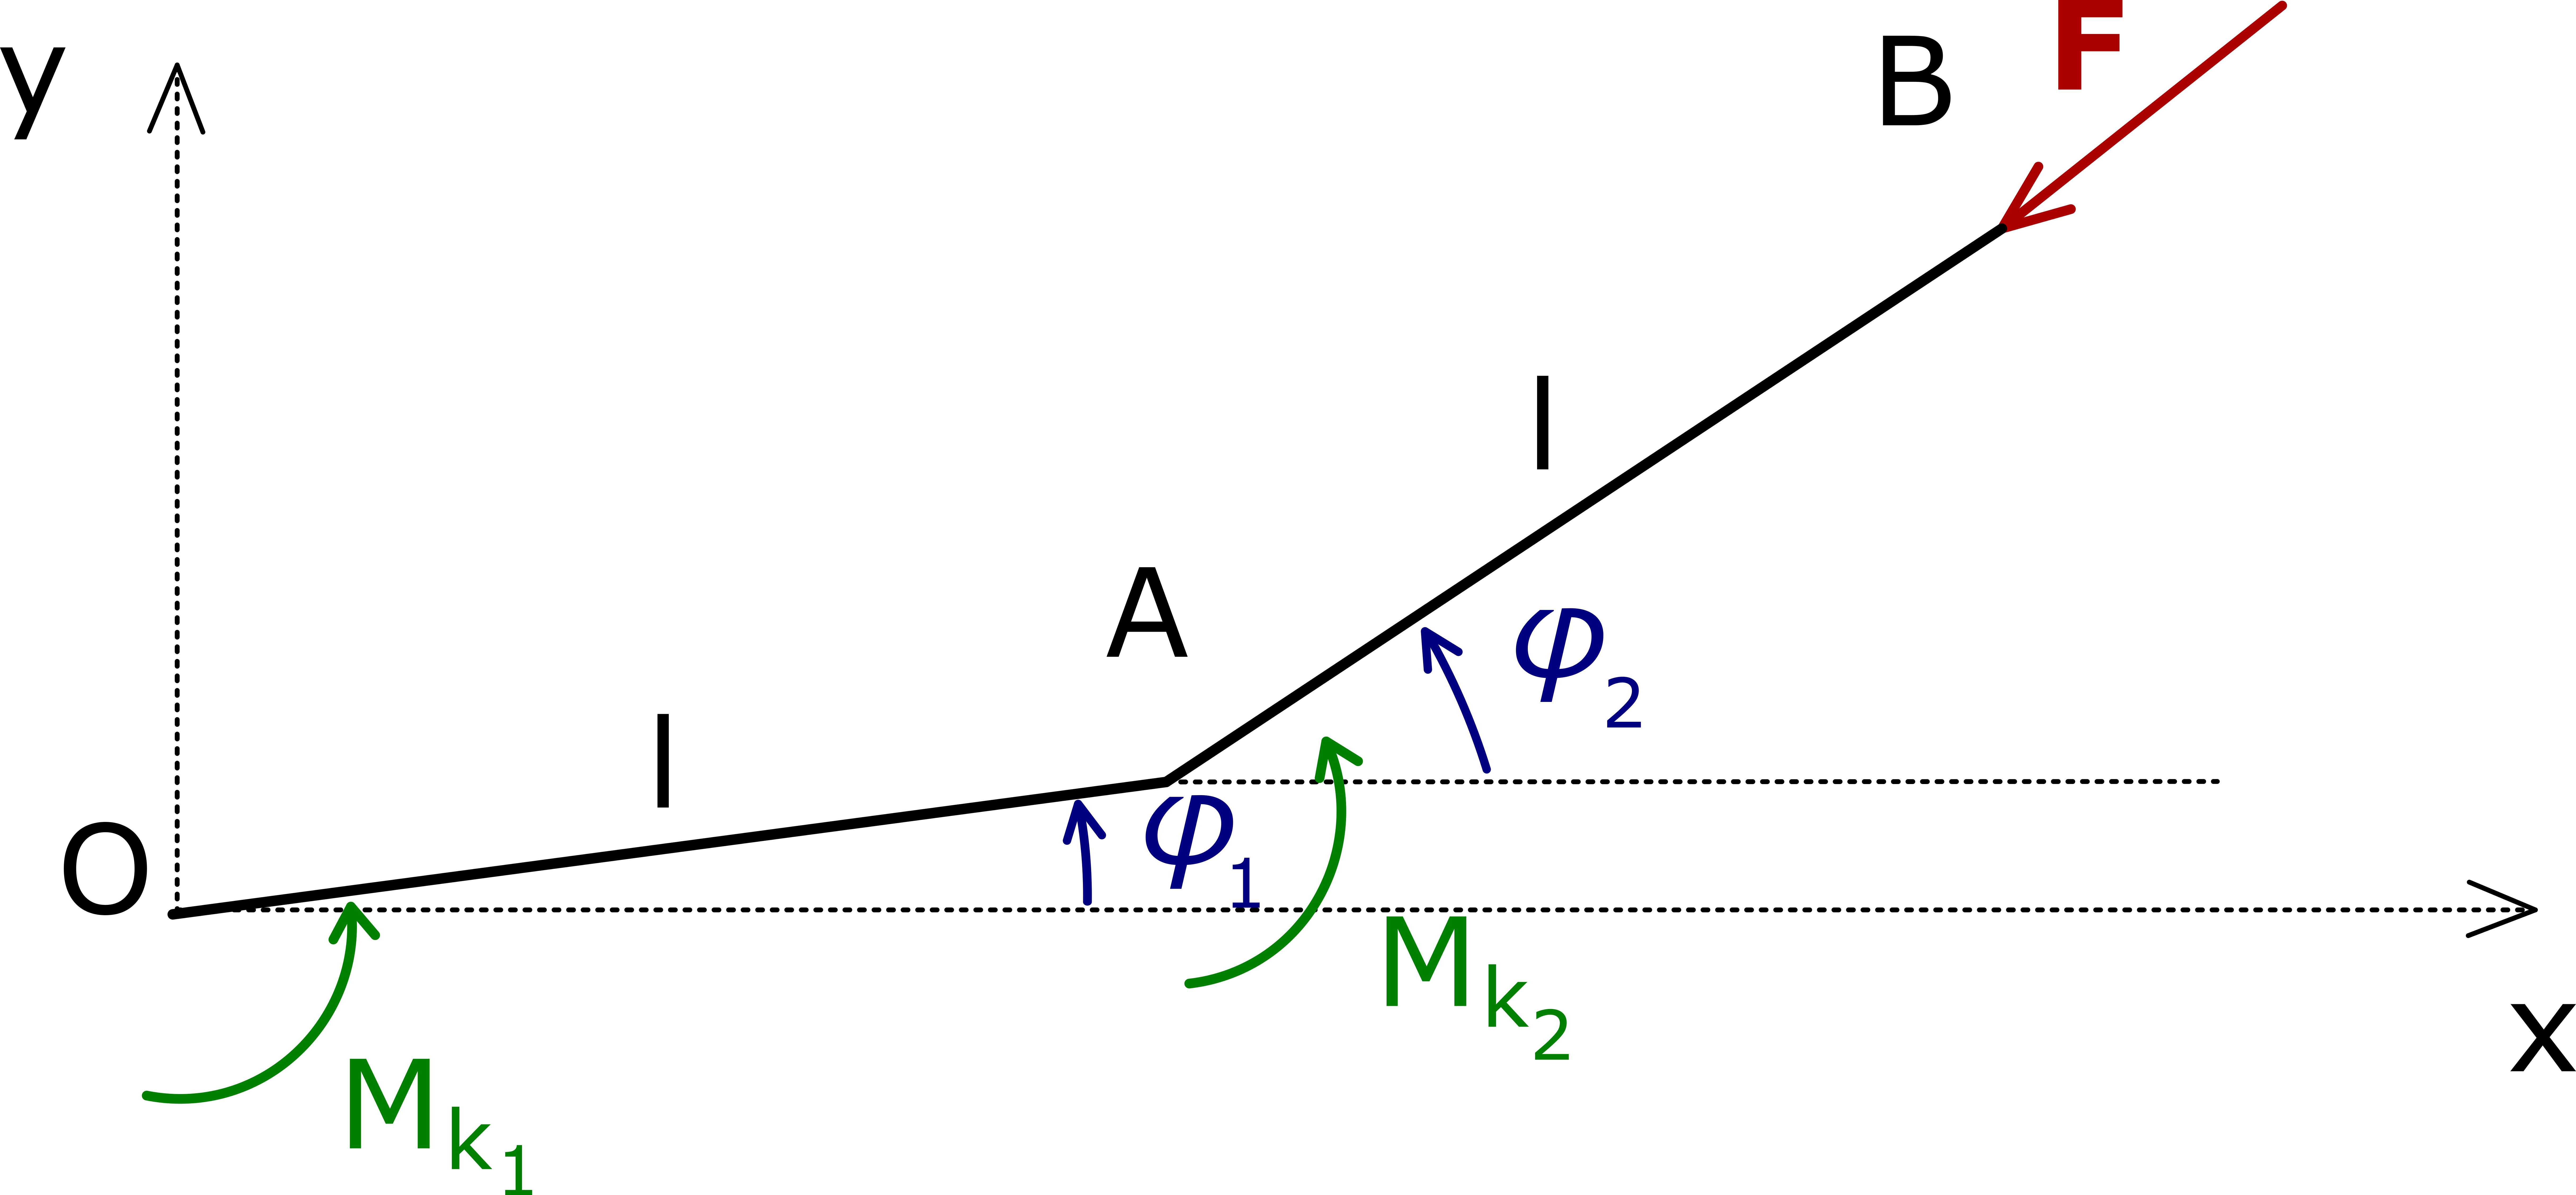
\includegraphics[scale=1]{2szab_koveto}
\end{figure}
 Jelölje a rugók merevségét $  k_1=k_2=k>0 $, a rúdak tömegét $  m_1=m_2=m>0 $, a rúdak hosszát $  l_1=l_2=l>0 $, az erő nagyságát \emph{F}. Legyen $  k>0, m>0, l>0, F>0 $ \newline
A rendszer mozgását a másodfokú Lagrange-egyenlet írja le.
\begin{equation} \label{eq:Newton}
\frac{d}{dt}\pd{T}{\dot\varphi_j}-\pd{T}{\varphi_j}+\pd{U}{\varphi_j}=q_j
\end{equation}
Ahol T a rendszer mozgási energiája, U a rugókban tárolt pontenciális energia, $\vec Q$ pedig a rendszer gerjesztése.

\subsection{Mozgási energia, potenciálix energia valamint a gerjesztés felírása}%2.1________________________
Mozgási energia:\newline
\begin{equation} \label{eq:Newton}
T(\vec\varphi)=\frac{1}{2 }\Theta_{1O}\dot\varphi_1^2+\frac{1}{2 }mv_{S_2}^2+\frac{1}{2 }\Theta_{2S_2}\dot\varphi_2^2,
\end{equation}
Ahol:
\begin{equation} \label{eq:Newton}
\Theta_{1O}=\frac{1}{3}ml^2; \; \quad \Theta_{2s}=\frac{1}{12}ml^2; \; \quad v_{2s}=\begin{bmatrix}
-\dot\varphi_1 l \sin (\varphi_1)-\dot\varphi_2 \frac{l}{2} \sin (\varphi_2)\\
\dot\varphi_1 l \cos (\varphi_1)+\dot\varphi_2 \frac{l}{2} \cos (\varphi_2)
\end{bmatrix}
\end{equation}
\begin{equation} \label{eq:Newton}
T(\vec\varphi)=ml^2\left(\frac{2}{3}\dot\varphi_1^2+\frac{1}{6}\dot\varphi_2^2+
\frac{1}{2}\dot\varphi_1\dot\varphi_2 \cos(\varphi_1-\varphi_2)\right)
\end{equation}
Potenciális energia:
\begin{equation} \label{eq:Newton}
U(\vec\varphi)=k/2 \cdot \varphi_1 ^2 + k/2 \cdot (\varphi_2-\varphi_1)^2=
k \cdot \varphi_1 ^2 + k/2 \cdot\varphi_2^2 -k \cdot \varphi_1\varphi_2
\end{equation}
Gerjesztés:
\begin{equation} \label{eq:Newton}
\vec Q(\vec\varphi)=[q_j]=\left[\vec F \cdot \frac{\partial \vec r_B}{\partial \varphi_j}\right]
\end{equation}
Ahol:
\begin{equation} \label{eq:Newton}
\vec F =
\begin{bmatrix}
-F \cos\varphi_2 \\
-F \sin\varphi_2
\end{bmatrix};\; \quad
\vec r_B=
\begin{bmatrix}
l(\cos\varphi_1+\cos\varphi_2)\\
l(\sin\varphi_1+\sin\varphi_2)
\end{bmatrix};
\end{equation}
\begin{equation} \label{eq:Newton}
\vec Q(\vec\varphi)=
\begin{bmatrix}
Fl\sin(\varphi_1-\varphi_2) \\
0
\end{bmatrix}
\end{equation}

\subsection{Linearizálás a $\vec\varphi=\vec0$ körül }%2.2______________
A másodfajú Lagrange egyenlet linearizálásval kapott mátrix differenciálegyenlet:
\begin{equation} \label{eq:Newton}
\vec M \vec{\ddot\varphi}+\vec K \vec{\varphi}=\vec Q
\end{equation}
Tömegmátrix:
\begin{equation} \label{eq:Newton}
\vec M(\vec\varphi)=[m_{i j}]=\left[\frac{\partial T}{\partial \dot\varphi_i  \partial \dot\varphi_j}\right]=
\end{equation}
\begin{equation} \label{eq:Newton}
\begin{bmatrix}
4/3 ml^2 & 1/2 ml^2\cos(\varphi_1-\varphi_2)\\
1/2 ml^2\cos(\varphi_1-\varphi_2) & 1/3 ml^2
\end{bmatrix}
\end{equation}
\begin{equation} \label{eq:Newton}
\vec M(\vec 0)=
\begin{bmatrix}
4/3 ml^2 & 1/2 ml^2 \\
1/2 ml^2 & 1/3 ml^2
\end{bmatrix}
\end{equation}
Merevségi mátrix:
\begin{equation} \label{eq:Newton}
\vec K(\vec\varphi)=[k_{ij}]=\left[\frac{\partial U}{\partial \varphi_i  \partial \varphi_j}\right]=
\begin{bmatrix}
2k & -k\\
-k & k
\end{bmatrix}
\end{equation}
Gerjesztés:
\begin{equation} \label{eq:Newton}
\vec Q(\vec\varphi) \approx \vec Q(\vec 0)+
\left[\frac{\partial \vec Q}{\partial \vec{\varphi}}\right]\vec{\varphi}=
\begin{bmatrix}
Fl &-Fl\\
0 & 0
\end{bmatrix} 
\begin{bmatrix}
\varphi_1\\
\varphi_2
\end{bmatrix} 
:= \vec K^{(F)} \vec \varphi
\end{equation}

A $\vec \varphi=\vec 0$ pont kis környezetében $\vec F$ erő konzervatívank tekinthető.{\color{blue} Lehetséges, hogy $\vec F$ erő $\vec \varphi=\vec 0$ pont kis környezetében, kismértékben ugyan, de növeli a rendszer energiáját, mely esetben a rendszer modellje semiképp sem lenne stabil. Azonban egy valós szerkezetnek mindig van csillapítása, melyet most az egyszerűség kedvéért 0-nak tekintek. Feltehető hogy $\vec \varphi=\vec 0$ pont megfelelően kis környezetében a rendszer energiájának $\vec F$ erő inkonzervativitása miatti növekedése kisebb mint a csillápítás miatti csökkenése, így ez az egyszerűsítés megtehető.\newline}A rendszer stabilitásának megállapításához elegedő $\vec F$ erő hatását is figyelembevevő  potenciálfüggvény vizsgálata.
\begin{equation} \label{eq:Newton}
\vec Q^{pot}(\vec\varphi) =[k_{i}]=\left[ \frac{\partial U}{\partial \varphi_i }\right]=
\begin{bmatrix}
2k \varphi_1 - k \varphi_2\\
k \varphi_2 - k \varphi_1
\end{bmatrix}
\end{equation}
\begin{equation}\label{eq:Newton}
\vec Q^{pot}(\vec 0)-\vec Q(\vec 0)=\vec 0
\end{equation}
\begin{equation} \label{eq:Newton}
\vec M(\vec 0) \vec{\ddot\varphi}+(\vec K(\vec 0)-\vec K^{F}) \vec{\varphi}=\vec 0
\end{equation}
Innen:
\begin{equation} \label{eq:Newton}
\vec K_0^*:=\vec K(\vec 0)-\vec K^{F}=
\begin{bmatrix}
2k-Fl & -k+Fl\\
-k & k
\end{bmatrix} 
\end{equation}
$\vec K_0^*$ előjeles aldeterminánsai:
\begin{equation} \label{eq:Newton}
K_0^*{aldet 1}=2k-Fl
\end{equation}
\begin{equation} \label{eq:Newton}
K_0^*{aldet 2}=(2k-Fl)(k)-(-k+Fl)(-k)=k^2
\end{equation}
$Fl>2k$ esetén $\vec \varphi=\vec 0$ pont instabil. Azonban ez a módszer nem vizsgálja a növekvő {\color{red}??? inkább nagy?} amplitúdójú rezgéseket, ezért $2k>Fl$ szükséges, de nem elégséges feltétele a stabilitásnak. {\color{red} lokális stabilitás vizsgálat?}
{\newline \color{blue} Itt arra gondoltam, hogy mivel a rendszernek nincs csillapítása, és a gerjesztése nem periodikus, ezért amikor konzervatívnak tekintettem F erőt, azzal egy olyan hibát tettem a modellembe ami integrálódhat is, ha a rendszer energiája szép lassan növekszik. Talán az alábbi megfogalmazás, a fenti kiegészítéssel jobb:\newline
$2k>Fl$ esetén $\vec \varphi=\vec 0$ pont stabil. Azonban nagy a amplitúdójú rezgések, vizsgálatához a linearizálás nem alkalmas.}

\subsection{Követő és nem követő erő esetén, kis amplitúdójú lengések lengésképének összehasonlítása}%2.3_____________
Legyen mindkét esetben m=1[kg], l=0,1 [m], F=10[N], k=5 [Nm/rad], így $\vec\varphi= \vec0$ midkét esetben stabil.\newline
A sajátkörfrekvenciáknak ($\omega_n$), és a hozzájuk tartozó sajátvektoroknak ($\vec A$) ki kell elégíteniük az alábbi mátrixegyenletet:

\begin{equation} \label{eq:Newton}
(-\omega_n^2 \matr M+\matr K) \vec A=\vec 0
\end{equation}
Ahol:
\begin{equation} \label{eq:Newton}
\vec A\neq \vec0; \quad A_1:=1
\end{equation}
Egy mátrixot nem nullvektorral szorozva akkor kaphatunk nullvektort, ha a mátrix determinánsa 0. Tehát:
\begin{equation} \label{eq:Newton}
det(-\omega_n^2 \matr M+\matr K)= 0
\end{equation}
Innen kiszámolhatóak a sajátkörfrekvenciák, melyek számossága a rendszer szabadsági fokaival egyezik meg. ($\omega_{n1} \leq \omega_{n2}$) Ezeket visszahelyettesítve az első egyenletbe megkaphatjuk a sajátvektorokat.\newline

\textbf{Állandó erővel gerjesztett rendszer:}
\begin{equation} \label{eq:Newton}
\matr M(\vec 0)=
\begin{bmatrix}
4/3 ml^2 & 1/2 ml^2 \\
1/2 ml^2 & 1/3 ml^2
\end{bmatrix}; \quad
\matr K(\vec0) =
\begin{bmatrix}
2k-Fl & -k \\
-k & k-Fl
\end{bmatrix}
\end{equation}
\begin{equation} \label{eq:Newton}
\omega_{n1}=9,13 [rad/s];\quad
\vec A_1=
\begin{bmatrix}
1 \\
-1,46
\end{bmatrix}[rad]
\end{equation}
\begin{equation} \label{eq:Newton}
\omega_{n2}=82,30 [rad/s];\quad
\vec A_2=
\begin{bmatrix}
1 \\
2,09
\end{bmatrix}[rad]
\end{equation}

{\color{blue} Furcsálom azt az eredményet. Én úgy éreztem, hogy az első sajátkörfrekvenciához tartozó lengésképnél lesz $A_2$ pozitív.}

\textbf{Követő erővel gerjesztett rendszer:}
\begin{equation} \label{eq:Newton}
\matr M(\vec 0)=
\begin{bmatrix}
4/3 ml^2 & 1/2 ml^2 \\
1/2 ml^2 & 1/3 ml^2
\end{bmatrix}; \quad
\matr K_0^* =
\begin{bmatrix}
2k-Fl & -k+Fl \\
-k & k
\end{bmatrix}
\end{equation}
\begin{equation} \label{eq:Newton}
\omega_{n1}=13,45 [rad/s];\quad
\vec A_1=
\begin{bmatrix}
1 \\
-1,34
\end{bmatrix}[rad]
\end{equation}
\begin{equation} \label{eq:Newton}
\omega_{n2}=84,29 [rad/s];\quad
\vec A_2=
\begin{bmatrix}
1 \\
2.17
\end{bmatrix}[rad]
\end{equation}
{\color{blue} A következő ábrákat sehogy sem tudtam szépre megcsinálni. Újra tervezem írni a scriptet pythonban. Ott nagyobb szabadságom van az ábrázolásban. A kék vonalak jelzik az első míg a pirosak a második sajátkörfrekvenciához tartozó lengésképeket.}
\begin{figure}[H]
\center
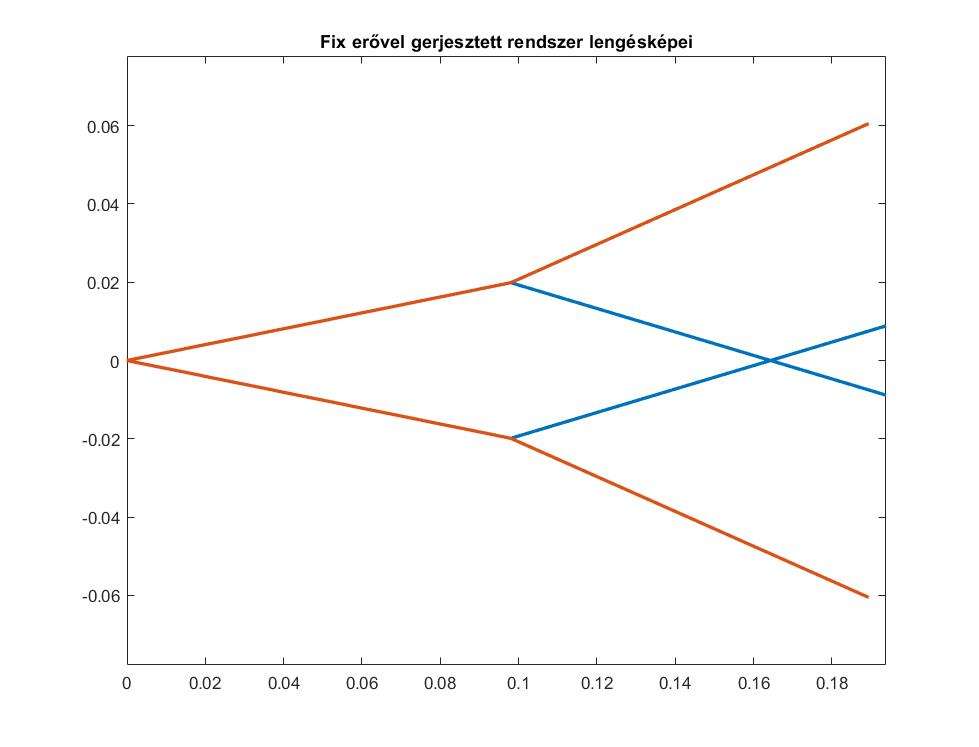
\includegraphics[scale=0.4]{lengésképek/fix_ero_lengeskep.jpg}
\end{figure}
\begin{figure}[H]
\center
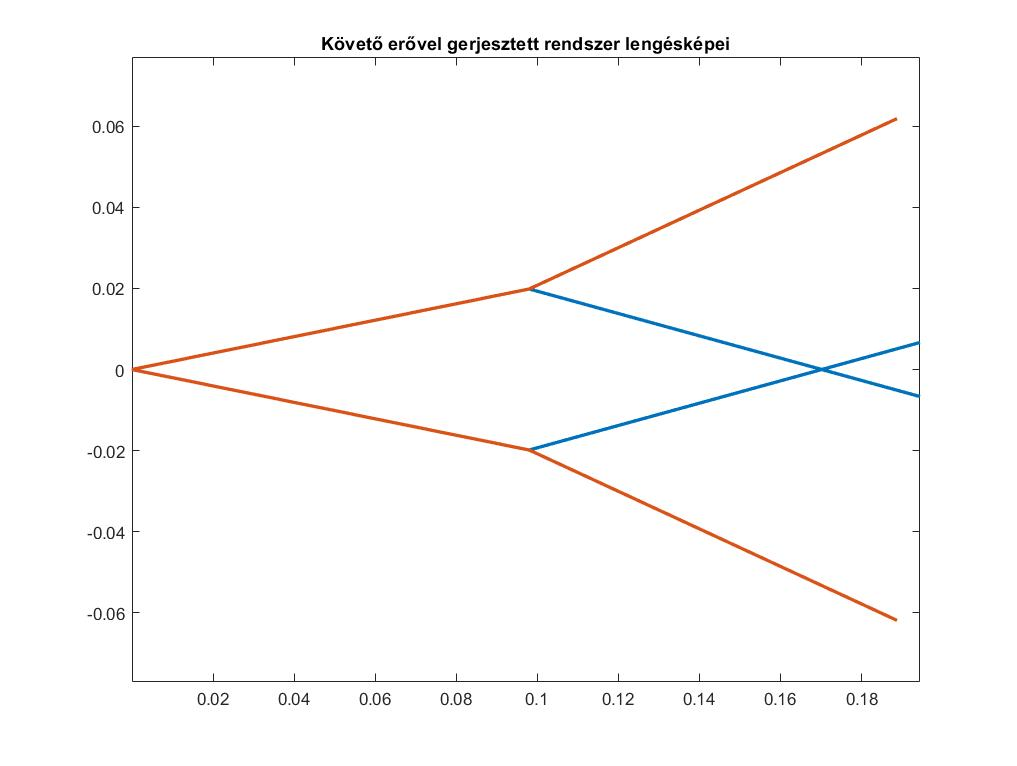
\includegraphics[scale=0.4]{lengésképek/koveto_ero_lengeskep.jpg}
\end{figure}

\subsection{Másodfokú Laplace egyenlet kifejtése}%2.4____________________________________________________
\begin{figure}[H]
\center
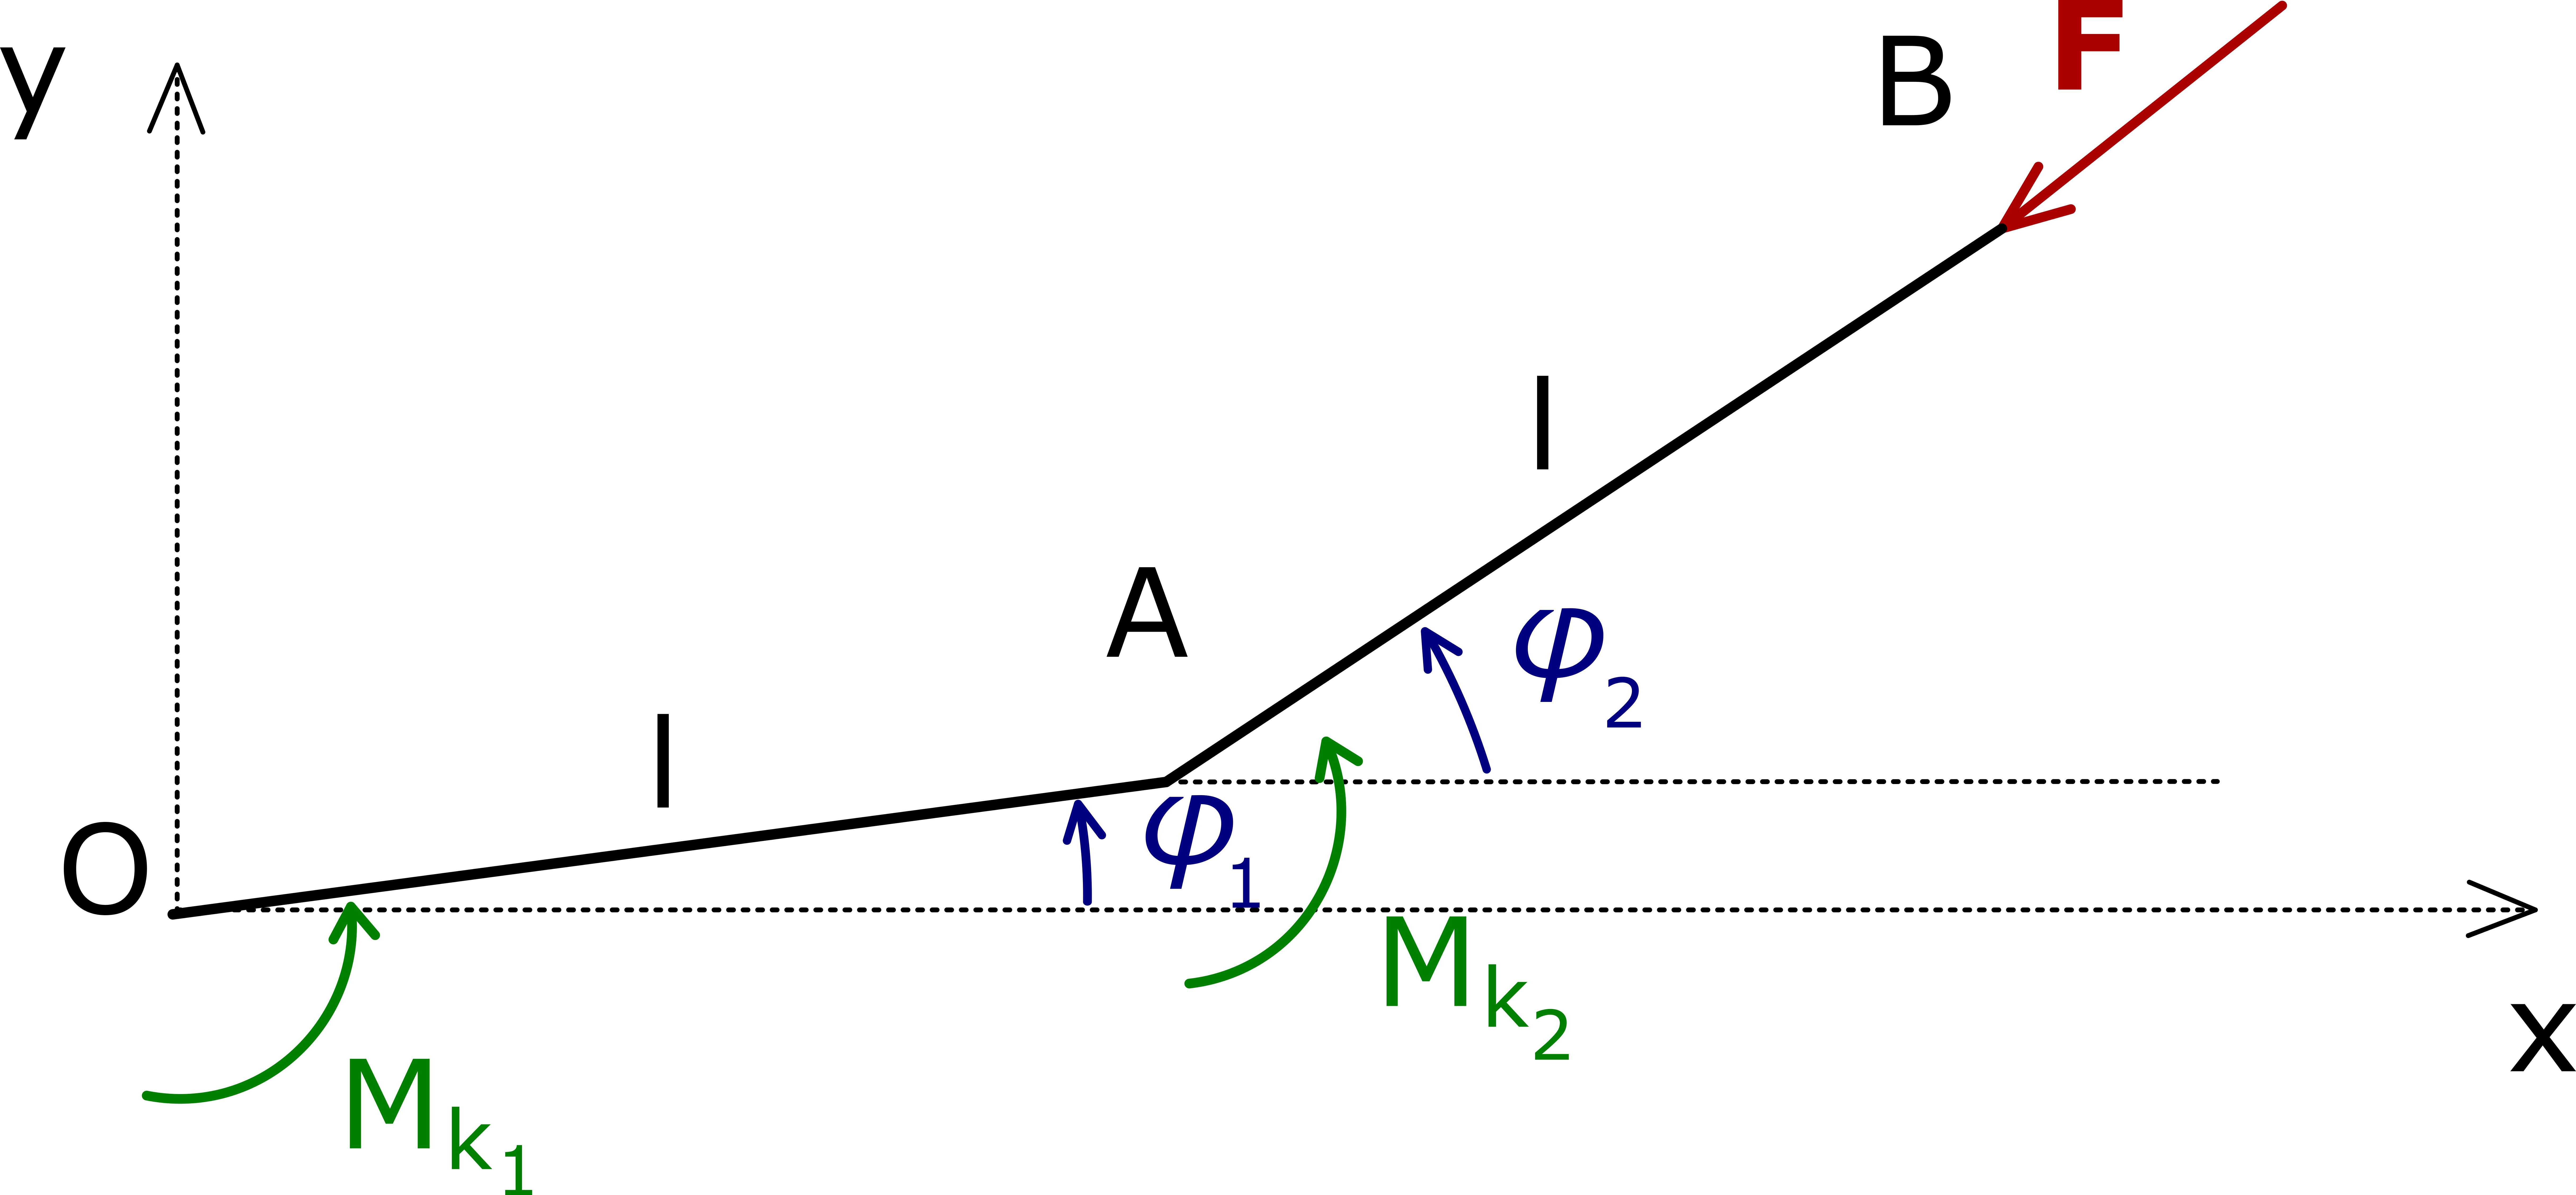
\includegraphics[scale=1]{2szab_koveto}
\end{figure}
Másodfokú Laplace egyenlet:
\begin{equation} \label{eq:Newton}
\frac{d}{dt}\frac{\partial T}{\partial \dot \varphi_i}-\frac{\partial T}{\partial \varphi_i}+\frac{\partial U}{\partial \varphi_i}=q_i
\end{equation}
A mozgási energia, pottenciális energia, és gerjesztés függvények:
\begin{equation} \label{eq:Newton}
T(\vec\varphi)=ml^2\left(\frac{2}{3}\dot\varphi_1^2+\frac{1}{6}\dot\varphi_2^2+
\frac{1}{2}\dot\varphi_1\dot\varphi_2 \cos(\varphi_1-\varphi_2)\right)
\end{equation}
\begin{equation} \label{eq:Newton}
U(\vec\varphi)=k \cdot \varphi_1 ^2 + k/2 \cdot\varphi_2^2 -k \cdot \varphi_1\varphi_2
\end{equation}
\begin{equation} \label{eq:Newton}
\vec Q(\vec\varphi)=
\begin{bmatrix}
Fl\sin(\varphi_1-\varphi_2) \\
0
\end{bmatrix}
\end{equation}
Az egyenlet kifejtése \newline
i=1:
\begin{equation} \label{eq:Newton}
\frac{d}{dt}\frac{\partial T}{\partial \dot \varphi_1}=
ml^2\left(\frac{4}{3} \ddot \varphi_1+\frac{1}{2}\ddot \varphi_2 \cos{(\varphi_1-\varphi_2)}+\dot\varphi_2^2\sin{(\varphi_1-\varphi_2)}-\dot\varphi_1\dot\varphi_2\sin{(\varphi_1-\varphi_2)}\right)
\end{equation}
\begin{equation} \label{eq:Newton}
-\frac{\partial T}{\partial \varphi_1}=ml^2\left(\dot\varphi_1\dot\varphi_2\sin{(\varphi_1-\varphi_2)}\right)
\end{equation}
\begin{equation} \label{eq:Newton}
\frac{\partial U}{\partial \varphi_1}=2k\varphi_1-k\varphi_2
\end{equation}
\begin{equation} \label{eq:Newton}
q_1 =Fl \sin{(\varphi_1-\varphi_2)}
\end{equation}
i=2:
\begin{equation} \label{eq:Newton}
\frac{d}{dt}\frac{\partial T}{\partial \dot \varphi_2}=
ml^2\left(\frac{1}{3} \ddot \varphi_2+\frac{1}{2}\ddot \varphi_1 \cos{(\varphi_1-\varphi_2)}-\dot\varphi_1^2\sin{(\varphi_1-\varphi_2)}+\dot\varphi_1\dot\varphi_2\sin{(\varphi_1-\varphi_2)}\right)
\end{equation}
\begin{equation} \label{eq:Newton}
-\frac{\partial T}{\partial \varphi_2}=-ml^2\left(\dot\varphi_1\dot\varphi_2\sin{(\varphi_1-\varphi_2)}\right)
\end{equation}
\begin{equation} \label{eq:Newton}
\frac{\partial U}{\partial \varphi_1}=k\varphi_2-k\varphi_1
\end{equation}
\begin{equation} \label{eq:Newton}
q_2 =0
\end{equation}
A kifejtett egyenletrendszer:
\begin{equation} \label{eq:Newton}
\begin{cases}
ml^2\left(\frac{4}{3} \ddot \varphi_1+\frac{1}{2}\ddot \varphi_2 \cos{(\varphi_1-\varphi_2)}+\dot\varphi_2^2\sin{(\varphi_1-\varphi_2)}\right)+2k\varphi_1-k\varphi_2=Fl \sin{(\varphi_1-\varphi_2)}
\\ 
ml^2\left(\frac{1}{3} \ddot \varphi_2+\frac{1}{2}\ddot \varphi_1 \cos{(\varphi_1-\varphi_2)}-\dot\varphi_1^2\sin{(\varphi_1-\varphi_2)}\right)+k\varphi_2-k\varphi_1=0
\end{cases}
\end{equation}

\end{document}
